\documentclass{article}
\usepackage[parfill]{parskip}
\usepackage[utf8]{inputenc}
\usepackage{amsmath}
\usepackage{amsthm} % for proofs
\usepackage{amssymb}
\usepackage{graphicx}
\usepackage{bm}
\usepackage[toc,page]{appendix}
\graphicspath{ {./images} }

\title{Kalman Filters and Least Squares}
\author{Dávid Iván}

\begin{document}

\maketitle

\tableofcontents

\newpage

\section{Weighted Least Squares}

We have a linear system to solve:

\begin{equation}
    Ax = b
\end{equation}

Where $A \in \mathbb{R}^{m \times n}$, $x \in \mathbb{R}^n$, $b \in \mathbb{R}^m$. When $A$ has more rows than columns ($m > n$), we don't (necessarily) have an exact solution. This is where we use least squares to get an approximate solution. $x_E$ is the solution to the Euclidean distance minimization:

\begin{equation}
\begin{split}
    x_E &= \text{argmin}_x || Ax-b ||^2\\
    &= \text{argmin}_x \left[ (Ax-b)^T (Ax-b) \right]\\
    &= (A^T A)^{-1}A^T b
\end{split}
\end{equation}

\begin{figure}[ht]
 \centering
  \includegraphics[width=200pt]{images/weighted_LS.png}
  \caption{difference between ordinary least squares and weighted least squares solution. We want to be close to $b$ either in terms of Euclidean distance or Mahalanobis distance.}
  \label{fig:EucMah}
\end{figure}


$x_M$ is the solution to the Mahalanobis distance minimization (the weighted least squares problem):

\begin{equation}
\begin{split}
    x_M &= \text{argmin}_x || Ax-b ||^2_R\\
    &= \text{argmin}_x \left[ (Ax-b)^T R^{-1} (Ax-b) \right]\\
    &= (A^T R^{-1} A)^{-1}A^T R^{-1} b
\end{split}
\end{equation}

This can be justified when the residual is thought of as a Gaussian random variable with zero mean and covariance $R$:

\begin{equation}
    Ax - b = r \propto N(0, R)
\end{equation}

Of course, when $R$ covariance matrix is the identity, then the two solutions are the same: $x_E = x_M$. Figure \ref{fig:EucMah} shows the difference between $x_E$ and $x_M$.

\subsection{Block Least Squares}

Solving
\begin{equation}
    \text{argmin}_x \left[||A_1 x - b||^2_{R_1} + ||A_2 x - b||^2_{R_2}\right]
\end{equation}

is equivalent to solving the following "normal" weighted least squares problem.

Let's divide up the matrices $A$, $b$ and $R$ as shown on Figure \ref{fig:BlockLS}.

\begin{figure}[ht]
 \centering
  \includegraphics[width=200pt]{images/factor_LS_p1.png}
  \caption{weighted least squares with block matrices}
  \label{fig:BlockLS}
\end{figure}


$A_1 \in \mathbb{R}^{m_1 \times n}$, $A_2 \in \mathbb{R}^{m_2 \times n}$, $m_1 + m_2 = m$. $b_1 \in \mathbb{R}^{m_1}$, $b_2 \in \mathbb{R}^{m_2}$. $R_1 \in \mathbb{R}^{m_1 \times m_1}$, $Q_2 \in \mathbb{R}^{m_2 \times m_2}$. $R_1$ and $R_2$ are both positive (semi)definite matrices.

The WLS solution is

\begin{equation}
    x^* = (A^T R^{-1} A)^{-1} A^T R^{-1} b
\end{equation}

Figure \ref{fig:BlockLS2} shows how to calculate $A^T R^{-1}$

\begin{figure}[ht]
 \centering
  \includegraphics[width=200pt]{images/factor_LS_p2.png}
  \caption{Calculating the matrix $A^T R^{-1}$}
  \label{fig:BlockLS2}
\end{figure}

Now the WLS solution can be calculated as follows:

\begin{equation}
    x^* = (A^T_1 R^{-1}_1 A_1 + A^T_2 R^{-2}_2 A_2)^{-1} (A^T_1 R^{-1}_1 b_1 + A^T_2 R^{-2}_2 b_2)
\end{equation}

Now let's solve the following minimization problem:

\begin{equation}
    x^*_2 = \text{argmin}_x \left[||A_1 x - b||^2_{R_1} + ||A_2 x - b||^2_{R_2}\right] = \text{argmin} \left[ L_1(x) + L_2(x) \right]
\end{equation}

First calculate the derivative:

\begin{equation}
    \frac{d}{dx} (L_1(x) + L_2(x)) = 2(A_1 x - b_1)^T R^{-1}_1 A_1 + 2(A_2 x - b_2)^T R^{-1}_2 A_2
\end{equation}

Setting it to zero and solving it:

\begin{equation}
    \begin{split}
        2(A_1 x - b_1)^T R^{-1}_1 A_1 + 2(A_2 x - b_2)^T R^{-1}_2 A_2 = 0\\
        A^T_1 R^{-1}_1 (A_1 x - b_1) + A^T_2 R^{-1}_2 (A_2 x - b_2) = 0\\
        A^T_1 R^{-1}_1 A_1 x - A^T_1 R^{-1}_1 b_1 + A^T_2 R^{-1}_2 A_2 x - A^T_2 R^{-1}_2 b_2 = 0\\
        A^T_1 R^{-1}_1 A_1 x + A^T_2 R^{-1}_2 A_2 x = A^T_1 R^{-1}_1 b_1 + A^T_2 R^{-1}_2 b_2 \\
        (A^T_1 R^{-1}_1 A_1 + A^T_2 R^{-1}_2 A_2) x = A^T_1 R^{-1}_1 b_1 + A^T_2 R^{-1}_2 b_2 \\
        x^*_2 = (A^T_1 R^{-1}_1 A_1 + A^T_2 R^{-1}_2 A_2)^{-1} (A^T_1 R^{-1}_1 b_1 + A^T_2 R^{-1}_2 b_2)
    \end{split}
\end{equation}

Now we see that indeed, $x^*_2 = x^*$.

\section{Matrix inversion}

Let's calculate the following matrix inversion.

\begin{figure}[ht]
 \centering
  \includegraphics[width=200pt]{images/matrix_inversion.png}
\end{figure}

Where $D_1 \in \mathbb{R}^{N\times N}$, symmetric, invertible. $D_2 \in \mathbb{R}^{n\times n}$, symmetric, invertible. $E \in \mathbb{R}^{N\times n}$.

It is easy to derive the following expressions:

\begin{equation}
    \Delta_2 = (D_2 - E^T D^{-1}_1 E)^{-1}
\end{equation}

\begin{equation}
\begin{split}
    \Delta_1 &= D^{-1}_1 + D^{-1}_1 E \Delta_2 E^T D^{-1}_1\\
    &= (D_1 - E D^{-1}_2 E^T)^{-1}
\end{split}
\end{equation}

\begin{equation}
    \beta = -D^{-1}_1 E \Delta_2
\end{equation}

Note that if $N >> n$ and we already know $D^{-1}_1$ (calculated earlier), then we might use the first formulae for $\Delta_1$, instead of the second, where we would have to invert a big ($N \times N$) matrix.

\end{document}